\section{Dynamic Models}

\subsection{Use Case Sequence Diagrams}
\subsubsection{CreateSale Sequence Diagram}
\begin{figure}[H]
	\centering
		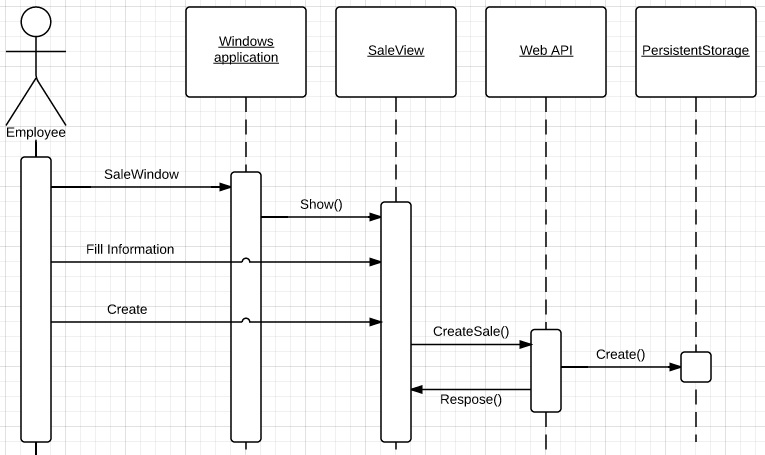
\includegraphics[width=\textwidth]{Figures/SequenceDiagram-CreateSale}\\
		% place the figure in the Figures folder (located with the main file)
		% you need to fix the scale a few times to get it right, but latex does not compress so one can always zoom in to see details.
	\caption{Sequence diagram of the CreateSale use case.}
  \label{fig:SequenceDiagram-CreateSale}
  % label it something meanfull
\end{figure}

Sequence diagram \ref{fig:SequenceDiagram-CreateSale} is made from the use case \texttt{CreateSale UC-1}. \textit{Sec. \ref{create-order-use-case}}. \\\\
In this use case, the employee starts with opening the \texttt{DriveIT Windows Client}, and thereafter navigates to the \texttt{Sale} view. In the \texttt{Sale} view, the employee fills in the information necessary to create a \texttt{Sale}, and after the \texttt{Employee} has finished filling in the information, he or she clicks on the "Create" button.

The sale will then be created and saved in the persistent storage. The \texttt{Employee} will then be prompted with a pop-up window, telling if the save was a success or an error has occurred.

\subsubsection{CreateUserAccount Sequence Diagram}
\begin{figure}[H]
	\centering
		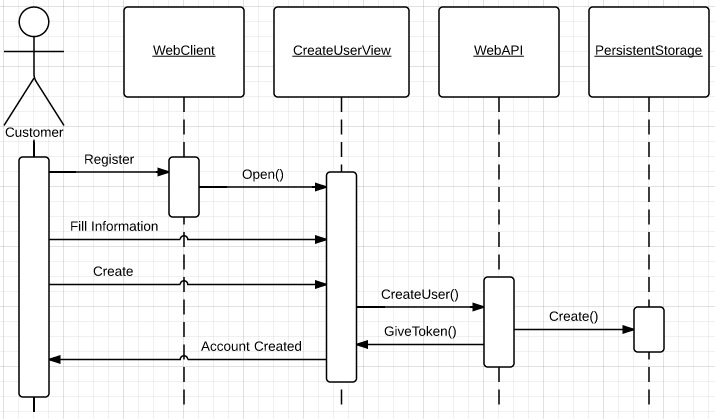
\includegraphics[width=\textwidth]{Figures/SequenceDiagram-CreateUserAccount}\\
		% place the figure in the Figures folder (located with the main file)
		% you need to fix the scale a few times to get it right, but latex does not compress so one can always zoom in to see details.
	\caption{Sequence diagram of the CreateUserAccount use case.}
  \label{fig:SequenceDiagram-CreateUserAccount}
  % label it something meanfull
\end{figure}

Sequence diagram \ref{fig:SequenceDiagram-CreateUserAccount} is made from the use case \texttt{CreateUserAccount UC-2}. \textit{Sec. \ref{create-account-use-case}}. \\\\
In this use case, the non-registered \texttt{Customer} has navigated to the \texttt{DriveIT Web Client}, clicks "Register", where after the customer is directed to the \texttt{CreateUserView}. 

In this view, the \texttt{Customer} will be filling in the necessary information, and \texttt{Customer} he or she then clicks the "Create" button. The \texttt{Customer} account will then be created and saved in the persistent storage. The \texttt{Customer} will then be redirected to the \texttt{DriveIT Web Client} front page and is logged in.

\subsubsection{ContactInterestedCustomer Sequence Diagram}
\begin{figure}[H]
	\centering
		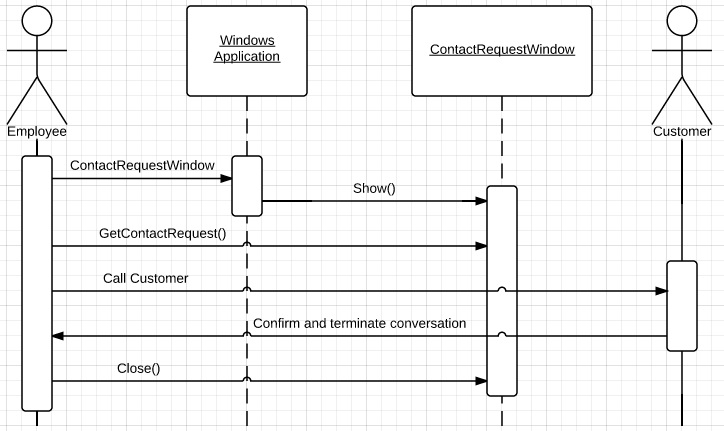
\includegraphics[width=\textwidth]{Figures/SequenceDiagram-ContactInterestedCustomer}\\
		% place the figure in the Figures folder (located with the main file)
		% you need to fix the scale a few times to get it right, but latex does not compress so one can always zoom in to see details.
	\caption{Sequence diagram of the ContactInterestedCustomer use case.}
  \label{fig:SequenceDiagram-ContactInterestedCustomer}
  % label it something meanfull
\end{figure}

Sequence diagram \ref{fig:SequenceDiagram-ContactInterestedCustomer} is made from the use case \texttt{ ContactInterested} \texttt{Customer UC-4} \textit{Sec. \ref{contact-interested-customer-use-case}}. \\\\
In this case, the \texttt{Employee} starts by opening the \texttt{DriveIT Windows Client}. The \texttt{Employee} then navigates to the \texttt{ContactRequestView}, where there will be shown a list of \texttt{Contact Requests} by different \texttt{Customers}. 

The \texttt{Employee} picks one of the \texttt{Contact Request} and a more detailed view of the \texttt{Contact Request} will be shown. The \texttt{Employee} navigates to the \texttt{CustomerView}, finds the specific \texttt{Customer} and finds his information by clicking on the \texttt{Customer}.

\subsubsection{RequestEmployeeContact Sequence Diagram}
\begin{figure}[H]
	\centering
		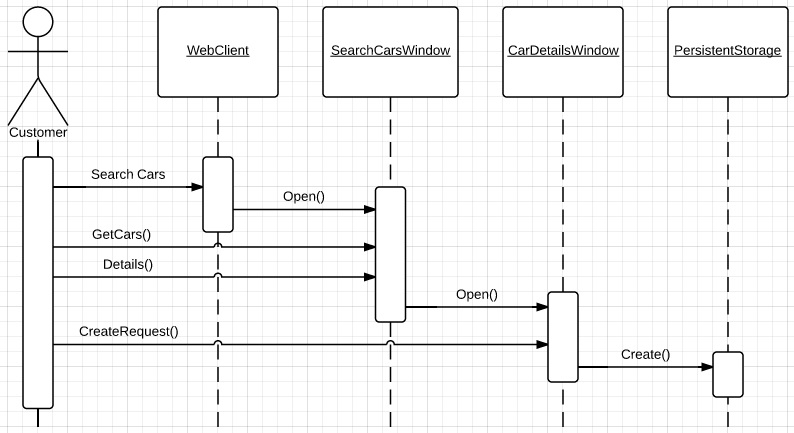
\includegraphics[width=\textwidth]{Figures/SequenceDiagram-RequestEmployeeContact}\\
		% place the figure in the Figures folder (located with the main file)
		% you need to fix the scale a few times to get it right, but latex does not compress so one can always zoom in to see details.
	\caption{Sequence diagram of the RequestEmployeeContact use case.}
  \label{fig:SequenceDiagram-RequestEmployeeContact}
  % label it something meanfull
\end{figure}

Sequence diagram \ref{fig:SequenceDiagram-RequestEmployeeContact} is made from the use case \texttt{ RequestEmployee} \texttt{Contact UC-5}. \textit{Sec. \ref{request-contact-use-case}}. \\\\
In this case, the \texttt{Customer} is signed in and has navigated to the \texttt{DriveIT Web Client} and then clicks "Find Cars", whereupon the "CarView" will be show. 

The \texttt{Customer} will then search for the specific \texttt{Car} that he or she is trying to find. The \texttt{Customer} will then navigate to the details of the \texttt{Car}, by clicking "Details". Then the \texttt{Customer} creates a request by clicking "Request to get contacted". The \texttt{Contact Request} will then be created and saved in the persistent storage.

\subsection{State Diagrams}
\subsubsection{Car State Diagram}
\begin{figure}[H]
	\centering
		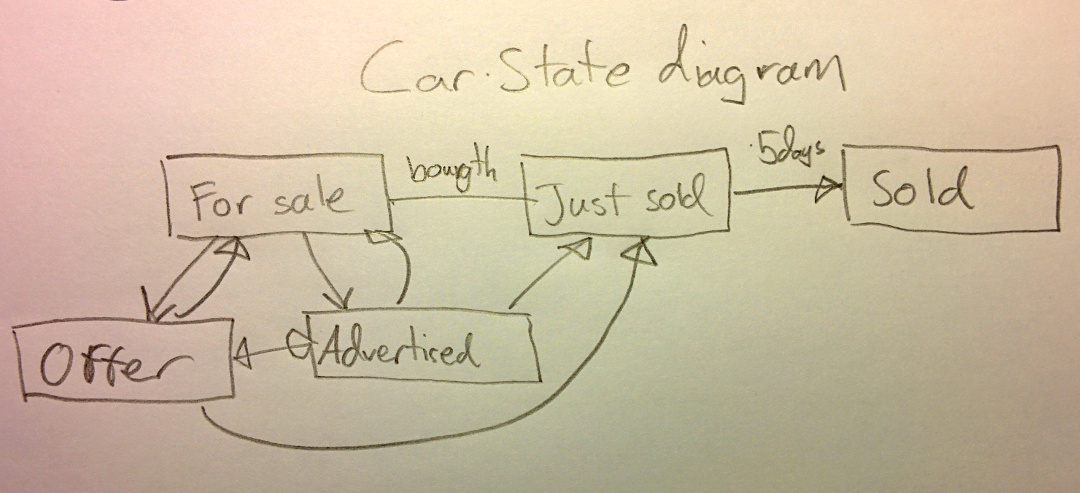
\includegraphics[width=\textwidth]{Figures/StateDiagram-Car}\\
		% place the figure in the Figures folder (located with the main file)
		% you need to fix the scale a few times to get it right, but latex does not compress so one can always zoom in to see details.
	\caption{State diagram of the Car object}
  \label{fig:StateDiagram-Car}
\end{figure}
Fig. \ref{fig:StateDiagram-Car} shows the states a \texttt{Car} can be in. It must always be possible to delete the \texttt{Car}, as shown in the diagram, but to be sold the \texttt{Car} must first enter the \textit{For Sale} state. 

In the \textit{For Sale} and \textit{Sold} state the \texttt{Car} should be visible from the \texttt{DriveIT Web Client} with a label indicating which of the two states it is in. The \texttt{Car} should not be visible on the \texttt{DriveIT Web Client} if sold more than a week ago. The \texttt{Car} should be visible from the \texttt{DriveIT Windows Client} in all of its states.\\